\pdfoutput=1
\documentclass[11pt]{article}

\usepackage[margin=1in]{geometry}
\usepackage{amsmath,amssymb,amsfonts}
\usepackage{booktabs}
\usepackage{graphicx}
\usepackage{hyperref}
\usepackage[numbers,sort&compress]{natbib}
\usepackage{microtype}

\title{Fisher--Rao Geometry as an Alternative to KL Divergence in t-SNE and Variational Autoencoders}

\author{
  Maruano T. Bottoni \\
  Independent Research Prototype \\
  \texttt{fisher-rao-ml}
}

\date{\today}

\begin{document}
\maketitle

\begin{abstract}
Many representation-learning objectives compare probability distributions with Kullback--Leibler
(KL) divergence. KL is computationally convenient, but it is asymmetric and its numerical scale is
not a metric distance on the statistical manifold. This report studies a preliminary replacement:
the Fisher--Rao geodesic distance. We implement differentiable Fisher--Rao objectives for
categorical distributions and diagonal Gaussian latent distributions, then test them in two
settings: a t-SNE-style neighborhood matching problem and a small MNIST variational autoencoder
(VAE). The results are early smoke tests rather than final empirical claims. They show that
Fisher--Rao objectives are trainable with PyTorch autograd, decrease smoothly under standard
optimizers, and act as a stronger VAE latent regularizer than KL at the same value of $\beta$.
We then evaluate final representation quality, geometry, and robustness under feature noise and
noisy inputs. In the compact t-SNE benchmark, Fisher--Rao improves several embedding metrics under
moderate-to-large feature noise. In the VAE benchmark, Fisher--Rao changes the reconstruction and
latent-geometry trade-off, with lower-$\beta$ Fisher--Rao improving latent kNN accuracy but not
noisy-input reconstruction.
\end{abstract}

\section{Introduction}

Distribution matching is a central operation in modern machine learning. In t-SNE, a low-dimensional
embedding is optimized so that its pairwise affinities match high-dimensional neighborhood
probabilities \citep{maaten2008visualizing}. In VAEs, an encoder distribution is regularized toward
a prior distribution while a decoder learns to reconstruct observations \citep{kingma2014auto}.
Both systems commonly use KL divergence.

This report asks a narrow research question:
\begin{quote}
Can Fisher--Rao distance replace or complement KL divergence in t-SNE and VAE objectives while
remaining trainable with standard gradient-based optimization?
\end{quote}

The motivation is geometric. The Fisher information matrix defines a Riemannian metric on a
statistical manifold \citep{fisher1925theory,rao1945information,amari2016information}. The induced
Fisher--Rao geodesic distance is symmetric and invariant to smooth reparameterizations. These
properties suggest that it may be a better comparison primitive when the object being compared is a
probability distribution rather than an arbitrary vector.

\section{Background}

\subsection{KL divergence}

For distributions $p$ and $q$ with common support, the KL divergence is
\begin{equation}
  \mathrm{KL}(p\|q) = \sum_i p_i \log \frac{p_i}{q_i}.
\end{equation}
KL is not symmetric and does not satisfy the triangle inequality. However, it is easy to estimate,
has strong variational interpretations, and is deeply embedded in probabilistic learning.

\subsection{Fisher--Rao distance on the simplex}

For categorical distributions, the square-root transform maps a probability vector $p$ to
$\sqrt{p}$ on the positive orthant of the unit sphere. Under the usual information-geometric
normalization, the Fisher--Rao distance between categorical distributions is
\begin{equation}
  d_{\mathrm{FR}}(p,q)
  = 2 \arccos\left(\sum_i \sqrt{p_i q_i}\right).
  \label{eq:categorical-fr}
\end{equation}
The experiments use $d_{\mathrm{FR}}(p,q)^2$ as the optimization objective. Figure
\ref{fig:categorical-shape} compares the two-class objective shape against KL.

\begin{figure}[t]
  \centering
  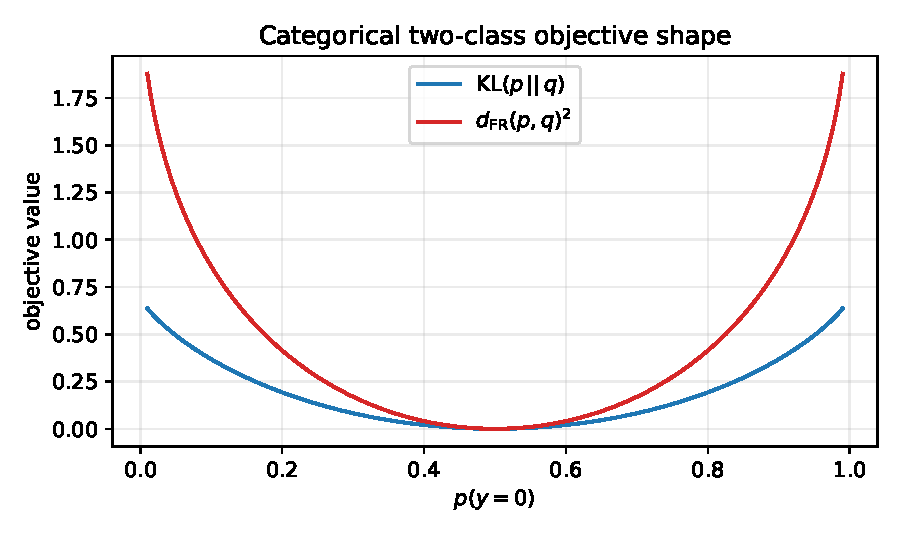
\includegraphics[width=0.68\linewidth]{figures/categorical_objective_shape.pdf}
  \caption{Objective shape for binary categorical distributions compared with a uniform target
  distribution. Fisher--Rao squared and KL have similar local behavior near the target but different
  global scaling.}
  \label{fig:categorical-shape}
\end{figure}

\subsection{Fisher--Rao distance for diagonal Gaussians}

For the VAE prototype, each latent dimension is treated as an independent univariate Gaussian
manifold. The implementation uses a closed-form univariate Fisher--Rao distance and combines
dimensions by summing squared per-dimension geodesic lengths. This is a diagonal-product
approximation, not a full covariance Gaussian geometry. For a posterior
$q_\phi(z|x)=\mathcal{N}(\mu,\mathrm{diag}(\sigma^2))$ and a standard normal prior, the regularizer
is
\begin{equation}
  \mathcal{R}_{\mathrm{FR}}(x)
  =
  d_{\mathrm{FR}}\left(q_\phi(z|x), \mathcal{N}(0,I)\right)^2.
\end{equation}
This replaces the standard VAE KL term
\begin{equation}
  \mathcal{R}_{\mathrm{KL}}(x)
  =
  \mathrm{KL}\left(q_\phi(z|x)\|\mathcal{N}(0,I)\right).
\end{equation}

\section{Methods}

\subsection{t-SNE objective}

The high-dimensional affinities are produced with a Gaussian kernel and normalized to a probability
distribution $P$. The low-dimensional affinities are produced with a Student-$t$ kernel and
normalized to $Q(Y)$. The baseline minimizes
\begin{equation}
  \mathcal{L}_{\mathrm{KL}}(Y)=\mathrm{KL}(P\|Q(Y)).
\end{equation}
The Fisher--Rao variant minimizes
\begin{equation}
  \mathcal{L}_{\mathrm{FR}}(Y)=d_{\mathrm{FR}}(P,Q(Y))^2.
\end{equation}
Both losses are differentiated through PyTorch autograd.

\subsection{VAE objective}

The VAE uses a small fully connected encoder-decoder architecture on MNIST. The baseline objective is
\begin{equation}
  \mathcal{L}_{\mathrm{VAE,KL}}
  =
  \mathbb{E}_{q_\phi(z|x)}[-\log p_\theta(x|z)]
  +
  \beta\, \mathrm{KL}(q_\phi(z|x)\|p(z)).
\end{equation}
The Fisher--Rao variant is
\begin{equation}
  \mathcal{L}_{\mathrm{VAE,FR}}
  =
  \mathbb{E}_{q_\phi(z|x)}[-\log p_\theta(x|z)]
  +
  \beta\, d_{\mathrm{FR}}(q_\phi(z|x),p(z))^2.
\end{equation}

\subsection{Evaluation metrics}

Raw KL and Fisher--Rao losses are not directly comparable. The code therefore logs
objective-independent final-model metrics. For t-SNE, the main metrics are trustworthiness,
neighborhood recall, silhouette score, and kNN classification accuracy in embedding space. For VAEs,
the main metrics are held-out reconstruction, regularization, BCE per pixel, mean posterior norm,
average posterior variance, active latent units, and kNN accuracy in latent-mean space.

\subsection{Robustness protocol}

The robustness experiments intentionally perturb inputs rather than objective values. For t-SNE, the
high-dimensional features used to construct $P$ are corrupted with isotropic Gaussian noise at
standard deviations $0$, $0.5$, and $1.0$ times the clean feature standard deviation. The final
embedding is evaluated against the clean features and labels, so the metrics measure whether the
objective preserves clean structure when the affinity graph is noisy. For VAEs, the model is trained
on clean MNIST and evaluated both on clean inputs and on noisy inputs clipped to $[0,1]$, while the
reconstruction target remains the clean image.

\section{Preliminary Experiments}

\subsection{Setup}

The current experiments are smoke tests run on Apple Silicon MPS. The t-SNE experiment uses synthetic
Gaussian clusters with $180$ samples, $8$ input dimensions, $200$ optimization steps, and Adam with
learning rate $0.05$. The VAE experiment uses one short MNIST epoch over $4096$ training examples,
latent dimension $8$, batch size $128$, Adam with learning rate $10^{-3}$, and $\beta=1$.

\subsection{t-SNE training behavior}

Both t-SNE objectives decrease smoothly under the same optimizer. Because the objective scales are
different, Figure \ref{fig:tsne-loss} reports normalized losses.

\begin{figure}[t]
  \centering
  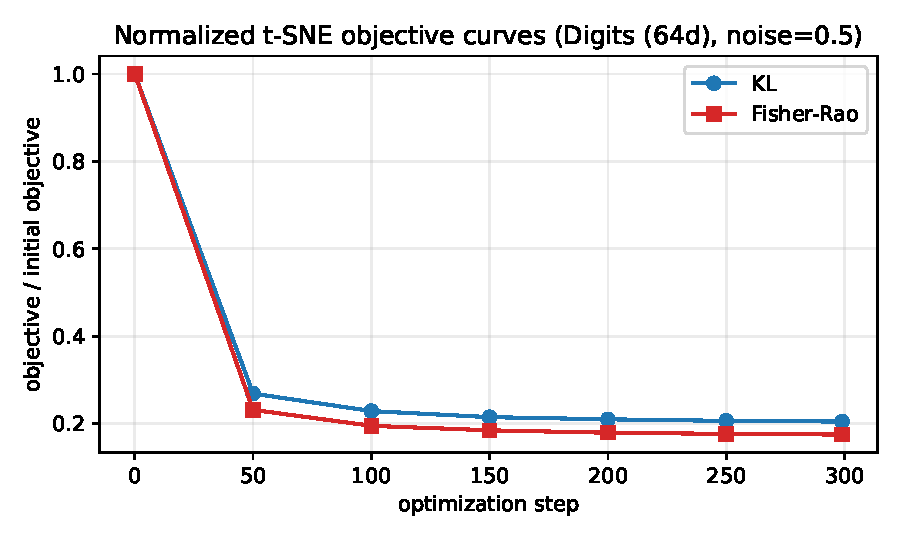
\includegraphics[width=0.72\linewidth]{figures/tsne_loss_curves.pdf}
  \caption{Normalized t-SNE objective curves. Both KL and Fisher--Rao squared decrease smoothly,
  which supports gradient feasibility. This does not by itself prove superior embedding quality.}
  \label{fig:tsne-loss}
\end{figure}

\begin{table}[t]
  \centering
  \caption{t-SNE smoke-run objective values.}
  \label{tab:tsne-loss}
  \begin{tabular}{lrrrrrr}
    \toprule
    Objective & Step 0 & Step 25 & Step 50 & Step 100 & Step 150 & Step 199 \\
    \midrule
    KL & 1.6131 & 0.6423 & 0.2989 & 0.1825 & 0.1419 & 0.1197 \\
    Fisher--Rao squared & 4.5652 & 1.8974 & 0.8964 & 0.5277 & 0.4069 & 0.3399 \\
    \bottomrule
  \end{tabular}
\end{table}

\subsection{VAE training behavior}

The VAE smoke run shows that both regularizers train without numerical instability. At the same
$\beta$, the Fisher--Rao regularizer is larger than the KL regularizer, suggesting that $\beta$
should be tuned separately for the two objectives.

\begin{figure}[t]
  \centering
  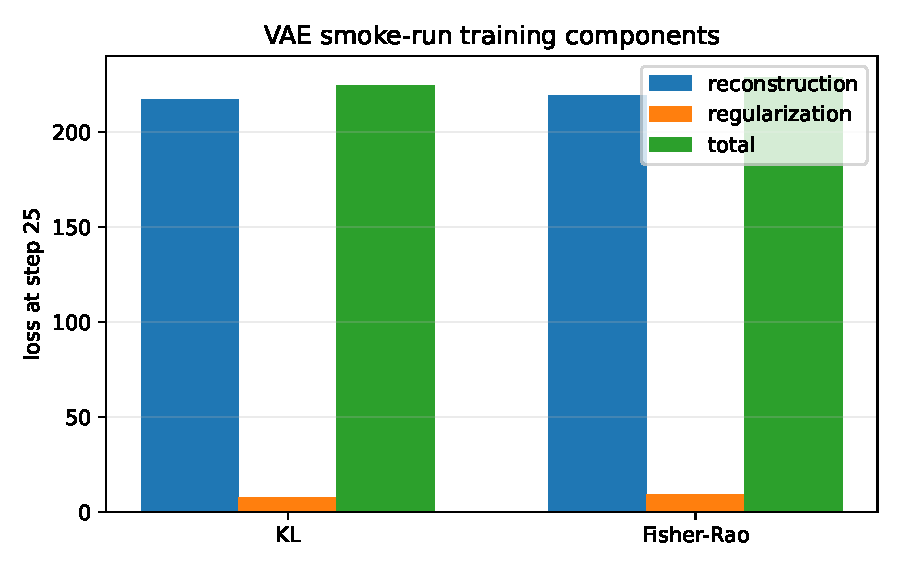
\includegraphics[width=0.72\linewidth]{figures/vae_training_components.pdf}
  \caption{VAE training components at step 25. Fisher--Rao produces a larger regularization term
  than KL at the same $\beta=1$, and the reconstruction term is slightly higher in this smoke run.}
  \label{fig:vae-components}
\end{figure}

\begin{table}[t]
  \centering
  \caption{VAE smoke-run metrics at step 25.}
  \label{tab:vae-step25}
  \begin{tabular}{lrrr}
    \toprule
    Regularizer & Total loss & Reconstruction & Regularization \\
    \midrule
    KL & 224.5261 & 216.8192 & 7.7069 \\
    Fisher--Rao & 228.4994 & 219.2852 & 9.2142 \\
    \bottomrule
  \end{tabular}
\end{table}

\section{Final Representation, Geometry, and Robustness}

The following compact benchmark directly addresses whether Fisher--Rao changes final model quality,
rather than only changing the training objective. These experiments are still small, but they test
the right axes: final representation quality, geometric neighborhood preservation, and robustness to
input corruption.

\subsection{t-SNE under feature noise}

Figure \ref{fig:tsne-robustness} and Table \ref{tab:tsne-robustness} evaluate t-SNE embeddings when
the high-dimensional features used to construct affinities are corrupted by increasing Gaussian
noise. Metrics are computed against the clean data. At zero noise, KL has slightly higher
trustworthiness and neighborhood recall, while Fisher--Rao has higher silhouette. Under moderate
noise ($0.5$), Fisher--Rao improves trustworthiness, neighborhood recall, silhouette, and kNN
accuracy. Under severe noise ($1.0$), Fisher--Rao improves trustworthiness, neighborhood recall, and
silhouette, while KL retains higher kNN accuracy.

\begin{figure}[t]
  \centering
  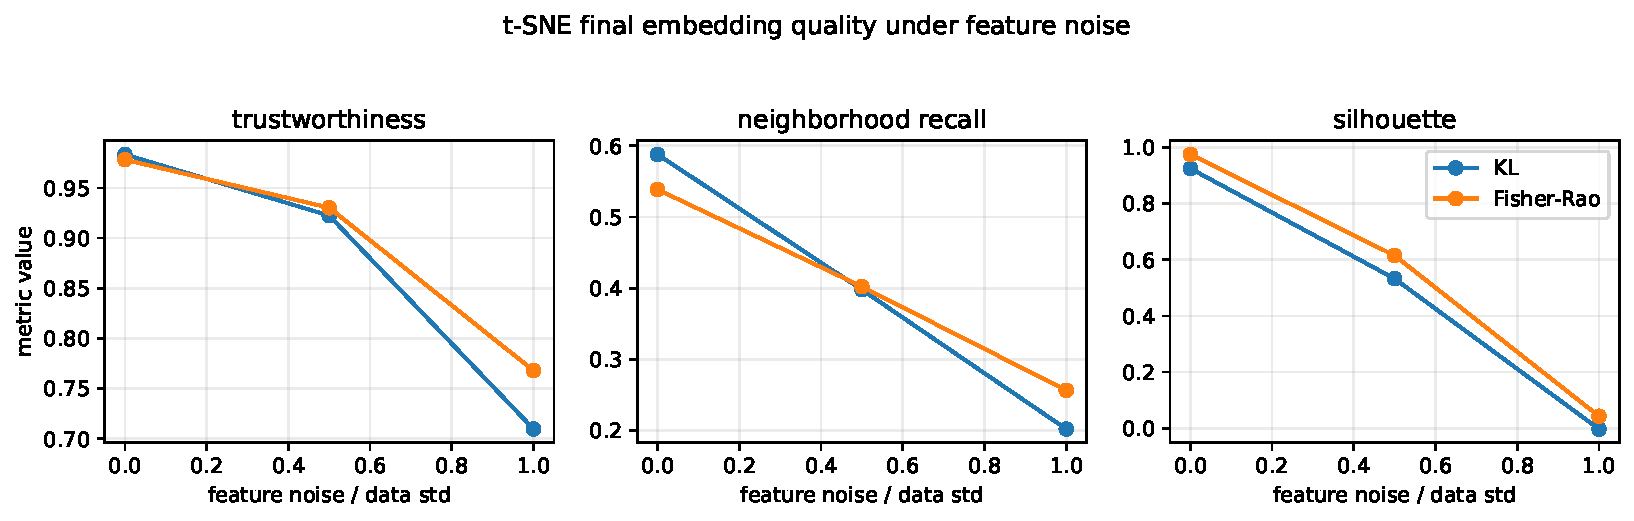
\includegraphics[width=\linewidth]{figures/tsne_robustness_metrics.pdf}
  \caption{Final t-SNE embedding metrics under feature noise. Noise is applied before constructing
  high-dimensional affinities, but metrics are computed against clean features and labels.}
  \label{fig:tsne-robustness}
\end{figure}

\begin{table}[t]
  \centering
  \caption{t-SNE robustness benchmark. Noise is expressed as a fraction of the clean feature
  standard deviation.}
  \label{tab:tsne-robustness}
  \begin{tabular}{llrrrr}
    \toprule
    Noise & Objective & Trust. & Recall & Silhouette & kNN acc. \\
    \midrule
    0.0 & KL & 0.9835 & 0.5879 & 0.9246 & 1.0000 \\
    0.0 & Fisher--Rao & 0.9782 & 0.5386 & 0.9746 & 1.0000 \\
    0.5 & KL & 0.9225 & 0.3979 & 0.5324 & 0.9286 \\
    0.5 & Fisher--Rao & 0.9303 & 0.4021 & 0.6149 & 0.9524 \\
    1.0 & KL & 0.7096 & 0.2021 & -0.0024 & 0.6667 \\
    1.0 & Fisher--Rao & 0.7679 & 0.2564 & 0.0431 & 0.6429 \\
    \bottomrule
  \end{tabular}
\end{table}

\subsection{VAE final metrics and noisy-input evaluation}

Figure \ref{fig:vae-final} and Table \ref{tab:vae-final} compare final VAE metrics after one compact
training run. Three settings are shown: KL with $\beta=1$, Fisher--Rao with the same $\beta=1$, and
Fisher--Rao with $\beta=0.3$. The lower-$\beta$ Fisher--Rao run improves latent kNN accuracy in this
small benchmark, but it also increases mean posterior norm and does not improve noisy-input
reconstruction. This supports the claim that Fisher--Rao changes the latent geometry trade-off, but
does not yet establish a general advantage.

\begin{figure}[t]
  \centering
  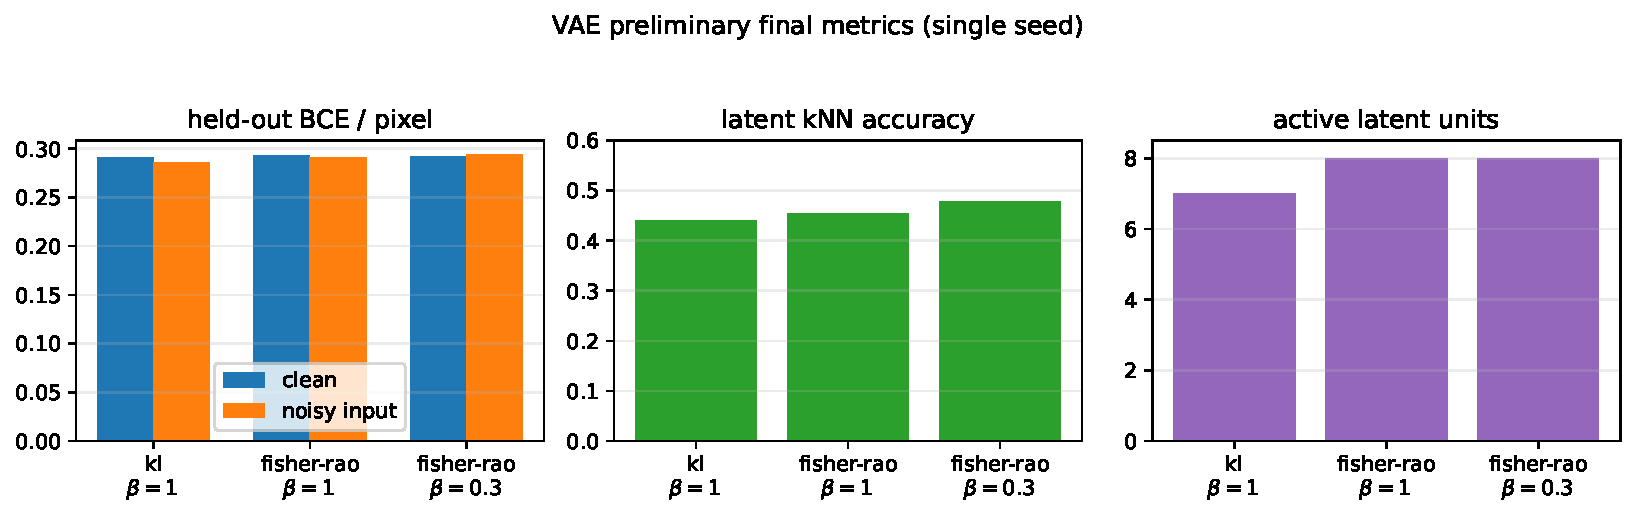
\includegraphics[width=\linewidth]{figures/vae_final_metrics.pdf}
  \caption{VAE final metrics. Fisher--Rao changes both reconstruction and latent representation
  behavior. Lowering $\beta$ improves latent kNN accuracy in this run, but noisy-input reconstruction
  is not improved.}
  \label{fig:vae-final}
\end{figure}

\begin{table}[t]
  \centering
  \caption{VAE final representation and robustness metrics.}
  \label{tab:vae-final}
  \begin{tabular}{llrrrrrr}
    \toprule
    Reg. & $\beta$ & BCE/pix & Noisy BCE & Mean norm & Var. mean & Active & Latent kNN \\
    \midrule
    KL & 1.0 & 0.2905 & 0.2864 & 5.5894 & 1.7532 & 7 & 0.4395 \\
    Fisher--Rao & 1.0 & 0.2930 & 0.2908 & 5.5915 & 2.6580 & 8 & 0.4551 \\
    Fisher--Rao & 0.3 & 0.2918 & 0.2938 & 7.1222 & 2.4461 & 8 & 0.4785 \\
    \bottomrule
  \end{tabular}
\end{table}

\section{Discussion}

The central positive result is feasibility. The categorical Fisher--Rao distance and the diagonal
Gaussian Fisher--Rao approximation produce finite gradients and can be optimized in the same
PyTorch training loops used for KL baselines. In the t-SNE prototype, replacing KL with
Fisher--Rao squared does not cause immediate optimization failure. In the VAE prototype,
Fisher--Rao behaves like a stronger latent penalty at $\beta=1$.

The final-metric benchmark gives a more useful, though still preliminary, signal. For t-SNE,
Fisher--Rao is competitive on clean data and appears more robust on several geometric metrics when
the affinity-building features are noisy. This is consistent with the geometric motivation: the
objective compares probability distributions through a symmetric geodesic distance rather than
through the asymmetric KL. For the VAE, the results are more mixed. Fisher--Rao activates more latent
dimensions and can improve latent kNN accuracy, but this comes with a larger posterior scale and no
clear reconstruction-robustness gain in the current setup.

The central caution is that lower raw loss is not the success criterion. KL and Fisher--Rao have
different units and numerical scales. A fair comparison should instead ask whether, after tuning
scale-sensitive hyperparameters, Fisher--Rao improves one of the following:
\begin{itemize}
  \item embedding neighborhood preservation or trustworthiness;
  \item stability across seeds;
  \item robustness under corrupted inputs;
  \item latent geometry and interpolation quality;
  \item avoidance of posterior collapse at comparable reconstruction quality.
\end{itemize}

\section{Limitations}

The experiments are preliminary. They use small datasets, short training horizons, and one seed for
the compact benchmark. The VAE Gaussian Fisher--Rao term uses a diagonal-product approximation
rather than a full covariance geodesic. The t-SNE experiment uses a simplified synthetic setup rather
than standard image features. Gradient clipping was used in the compact VAE benchmark after an
initial lower-$\beta$ Fisher--Rao run produced non-finite latent values. No claim of superiority over
KL should be made until the method is evaluated with multiple seeds, matched tuning budgets, and
downstream metrics.

\section{Next Experiments}

The next version should run the following protocol:
\begin{enumerate}
  \item Run KL and Fisher--Rao across $5$--$10$ random seeds.
  \item Tune $\beta$ separately for KL and Fisher--Rao in the VAE.
  \item Report mean and standard deviation for all objective-independent metrics.
  \item Add image reconstructions, generated samples, and latent interpolations to the report.
  \item Evaluate robustness under noisy or corrupted inputs.
\end{enumerate}

\section{Conclusion}

Fisher--Rao distance is a plausible geometric alternative to KL divergence for distribution-matching
objectives. The current implementation establishes differentiability and initial trainability in
t-SNE-style matching and VAE latent regularization. The strongest current observations are that
Fisher--Rao can improve some t-SNE geometric metrics under feature noise, and that it changes the
effective VAE latent-regularization geometry. Its practical value should be judged by final
representation quality, geometry, and robustness rather than by raw objective values.

\appendix

\section{Dataset and Corruption Details}

\subsection{Synthetic t-SNE data}

The compact robustness benchmark uses a synthetic five-cluster Gaussian dataset generated with
scikit-learn. The dataset has $140$ samples, $8$ input dimensions, cluster standard deviation $1.6$,
and random seed $101$. The clean feature matrix is denoted $X$. For each noise level
$\alpha \in \{0,0.5,1.0\}$, affinities are built from
\begin{equation}
  \widetilde{X}_\alpha = X + \alpha\, \mathrm{std}(X)\,\epsilon,
  \qquad \epsilon \sim \mathcal{N}(0,I).
\end{equation}
Final embedding metrics are computed against the clean $X$ and clean cluster labels. This separates
the training corruption from the evaluation target.

\subsection{MNIST VAE data}

The compact VAE benchmark uses MNIST with $2048$ training examples and $512$ held-out test examples.
Images are converted to tensors in $[0,1]$. Clean evaluation reconstructs clean inputs. Noisy
evaluation feeds
\begin{equation}
  \widetilde{x} = \mathrm{clip}(x + 0.25\,\epsilon,0,1),
  \qquad \epsilon \sim \mathcal{N}(0,I),
\end{equation}
to the encoder-decoder but computes reconstruction error against the clean target $x$.

\section{Training Dynamics Details}

\subsection{t-SNE benchmark dynamics}

All compact t-SNE benchmark runs use Adam with learning rate $0.05$, $120$ optimization steps,
Gaussian high-dimensional affinities with bandwidth $5.0$, and Student-$t$ low-dimensional
affinities. Table \ref{tab:appendix-tsne-dynamics} reports the recorded objective values.

\begin{table}[h]
  \centering
  \caption{t-SNE benchmark training dynamics.}
  \label{tab:appendix-tsne-dynamics}
  \begin{tabular}{llrrrrrrr}
    \toprule
    Noise & Objective & 0 & 20 & 40 & 60 & 80 & 100 & 119 \\
    \midrule
    0.0 & KL & 1.7032 & 0.9492 & 0.5978 & 0.3215 & 0.2560 & 0.2144 & 0.1881 \\
    0.0 & Fisher--Rao & 4.8845 & 3.0005 & 1.6774 & 0.9036 & 0.7072 & 0.6029 & 0.5364 \\
    0.5 & KL & 2.2743 & 1.6401 & 1.2104 & 0.9230 & 0.7859 & 0.7064 & 0.6554 \\
    0.5 & Fisher--Rao & 5.4343 & 4.0367 & 2.7401 & 2.1283 & 1.8484 & 1.6618 & 1.5377 \\
    1.0 & KL & 3.8903 & 3.2065 & 2.7303 & 2.4193 & 2.1722 & 2.0007 & 1.8705 \\
    1.0 & Fisher--Rao & 7.2506 & 6.4990 & 5.7426 & 5.1357 & 4.6848 & 4.3452 & 4.0951 \\
    \bottomrule
  \end{tabular}
\end{table}

\subsection{VAE benchmark dynamics}

All compact VAE benchmark runs use a fully connected encoder-decoder, latent dimension $8$, Adam
with learning rate $10^{-3}$, batch size $128$, one epoch, and gradient clipping at norm $10$. Table
\ref{tab:appendix-vae-dynamics} records the first logged training batch. Because the compact run has
only $16$ batches and logs every $20$ steps, the final comparison is made with held-out evaluation
metrics rather than the sparse training log.

\begin{table}[h]
  \centering
  \caption{VAE benchmark first logged training batch.}
  \label{tab:appendix-vae-dynamics}
  \begin{tabular}{llrrr}
    \toprule
    Regularizer & $\beta$ & Total loss & Reconstruction & Regularization \\
    \midrule
    KL & 1.0 & 552.1189 & 552.0860 & 0.0329 \\
    Fisher--Rao & 1.0 & 552.1514 & 552.0860 & 0.0654 \\
    Fisher--Rao & 0.3 & 552.1056 & 552.0860 & 0.0654 \\
    \bottomrule
  \end{tabular}
\end{table}

\bibliographystyle{plainnat}
\bibliography{references}

\end{document}
